\documentclass{beamer}
\usepackage{graphicx}
\graphicspath{{pictures/}}
\DeclareGraphicsExtensions{.pdf,.png,.jpg}
\usepackage[utf8x]{inputenc}
\usepackage[english,russian]{babel}
\usetheme{Madrid}


%Information to be included in the title page:
\title[] %optional
{Trading App. Приложение для прогнозирования стоимости акции с помощью анализа временных рядов.}

\subtitle{}

\author[Лукьяненеко И. А.] % (optional, for multiple authors)
{Лукьяненко Иван Андреевич, Б05-906}

\institute[MIPT] % (optional)
{
  Студент МФТИ ФПМИ 2 курс
}

\date[Python|ML 2021] % (optional)
{Проект по программированию.}

\begin{document}

\frame{\titlepage}
\begin{frame}


\frametitle{План презентации:}

 \begin{itemize}
  \item \textbf{Стек технологий:} используемые библиотеки и фреймворки;
  \item \textbf{Интерфейс приложения:} внешний вид и авторский дизайн;
  \item \textbf{Нейронная сеть:} структура нейронной сети, тренировочные и реальные данные;
  \item \textbf{Многопоточность:} где используются и зачем;
  \item \textbf{ООП и ФП:} использование ООП и Функционального Програмирования в проекте.
  \item \textbf{Подведение итогов:} контакты и дальнейшее развитие приложения.
 \end{itemize}

\end{frame}

\begin{frame}

 \frametitle{Стек технологий:}
 Стоит обозначить, что весь проект написан на Python 3.8\\
 В данном проекте использовались следующие библиотеки:
 \begin{itemize}
  \item \textbf{Интерфейс:} Tkinter;
  \item \textbf{Сбор данных и обработка данных:} yaml, numpy, pandas, pandas\_datareader, sklearn;
  \item \textbf{Нейронная сеть:} tensorlow;
  \item \textbf{Многопоточность:} threading;
  \item \textbf{Графики и изображния:} matplotlib, PIL
  \item \textbf{Дополнительно:} shutil, time
 \end{itemize}
 В репозитории с проектом лежит файл references.txt, где содержаться все библиотеки их версии.
\end{frame}

\begin{frame}
 \frametitle{Интерфейс приложения:}
 Основное окно:\\
 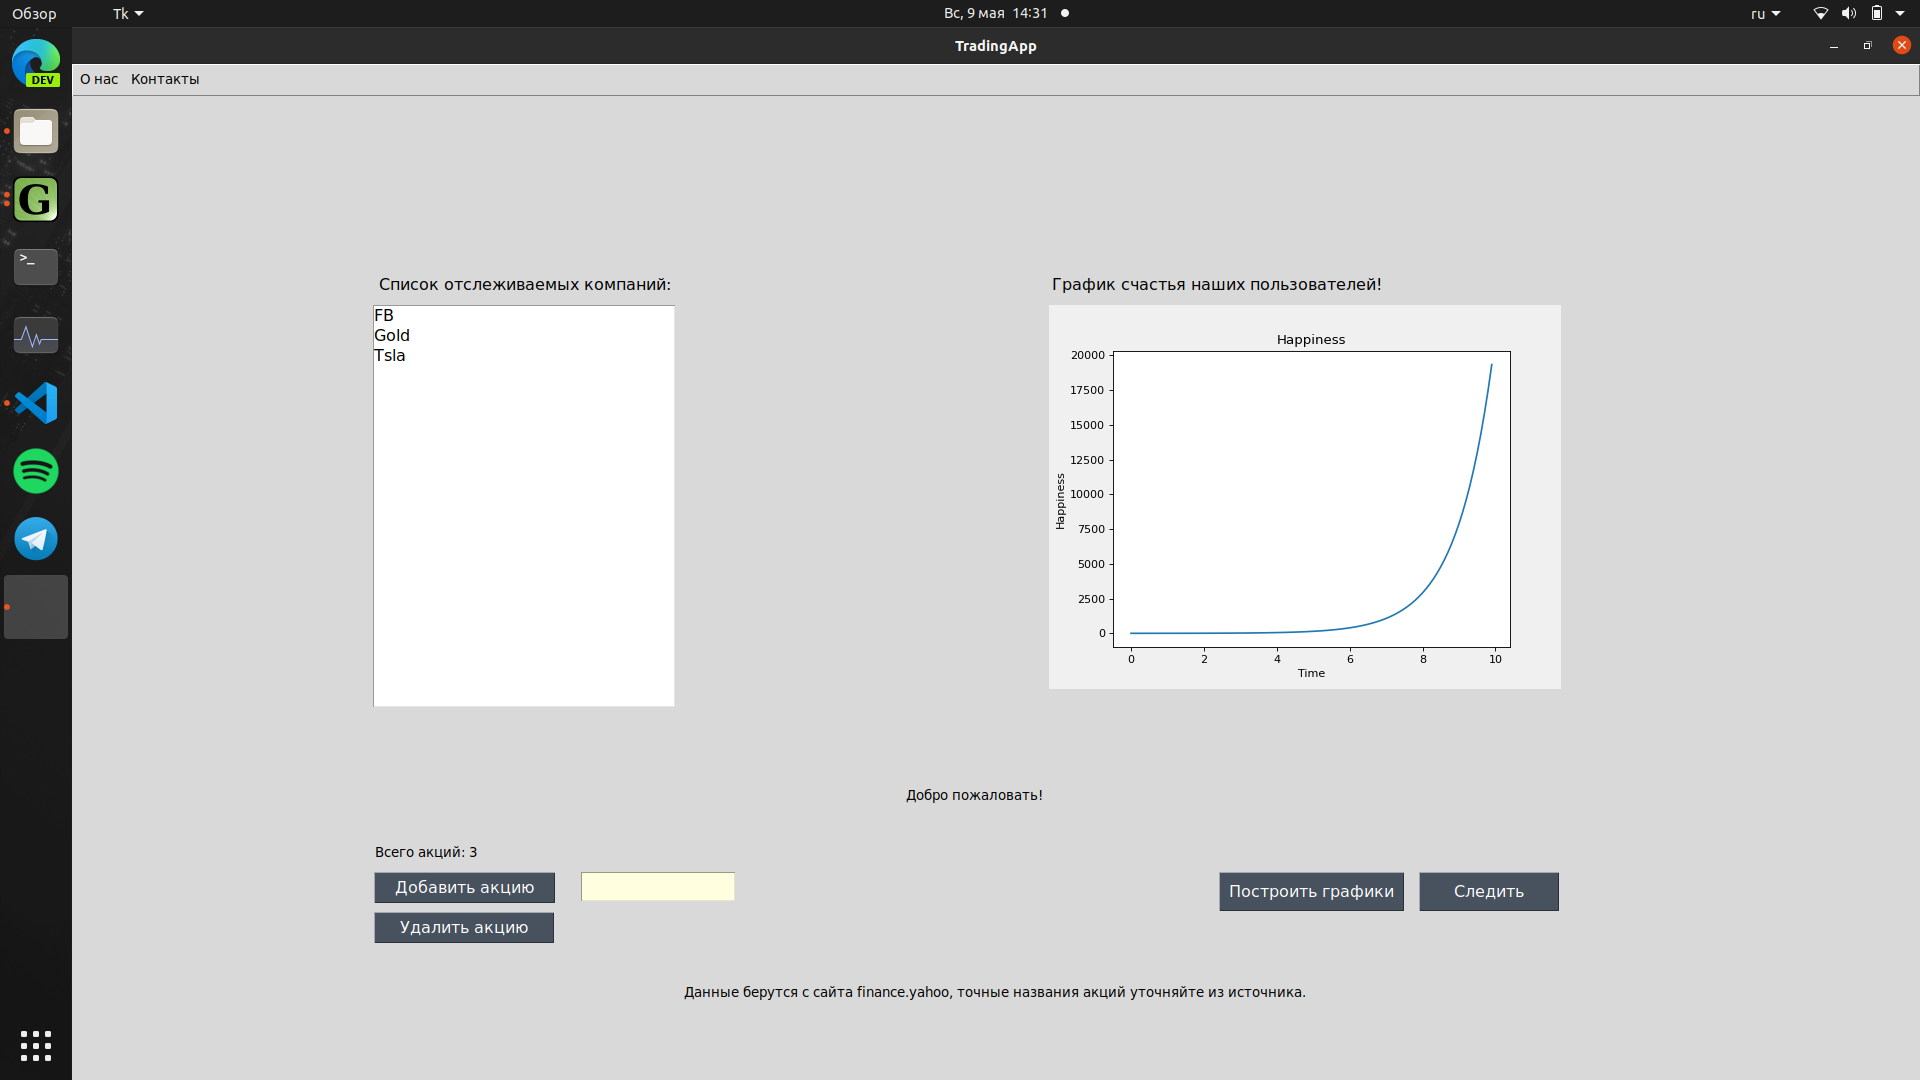
\includegraphics[scale=0.176]{mainWindow.png}
\end{frame}

\begin{frame}
 \frametitle{Интерфейс приложения:}
 О нас:\\
 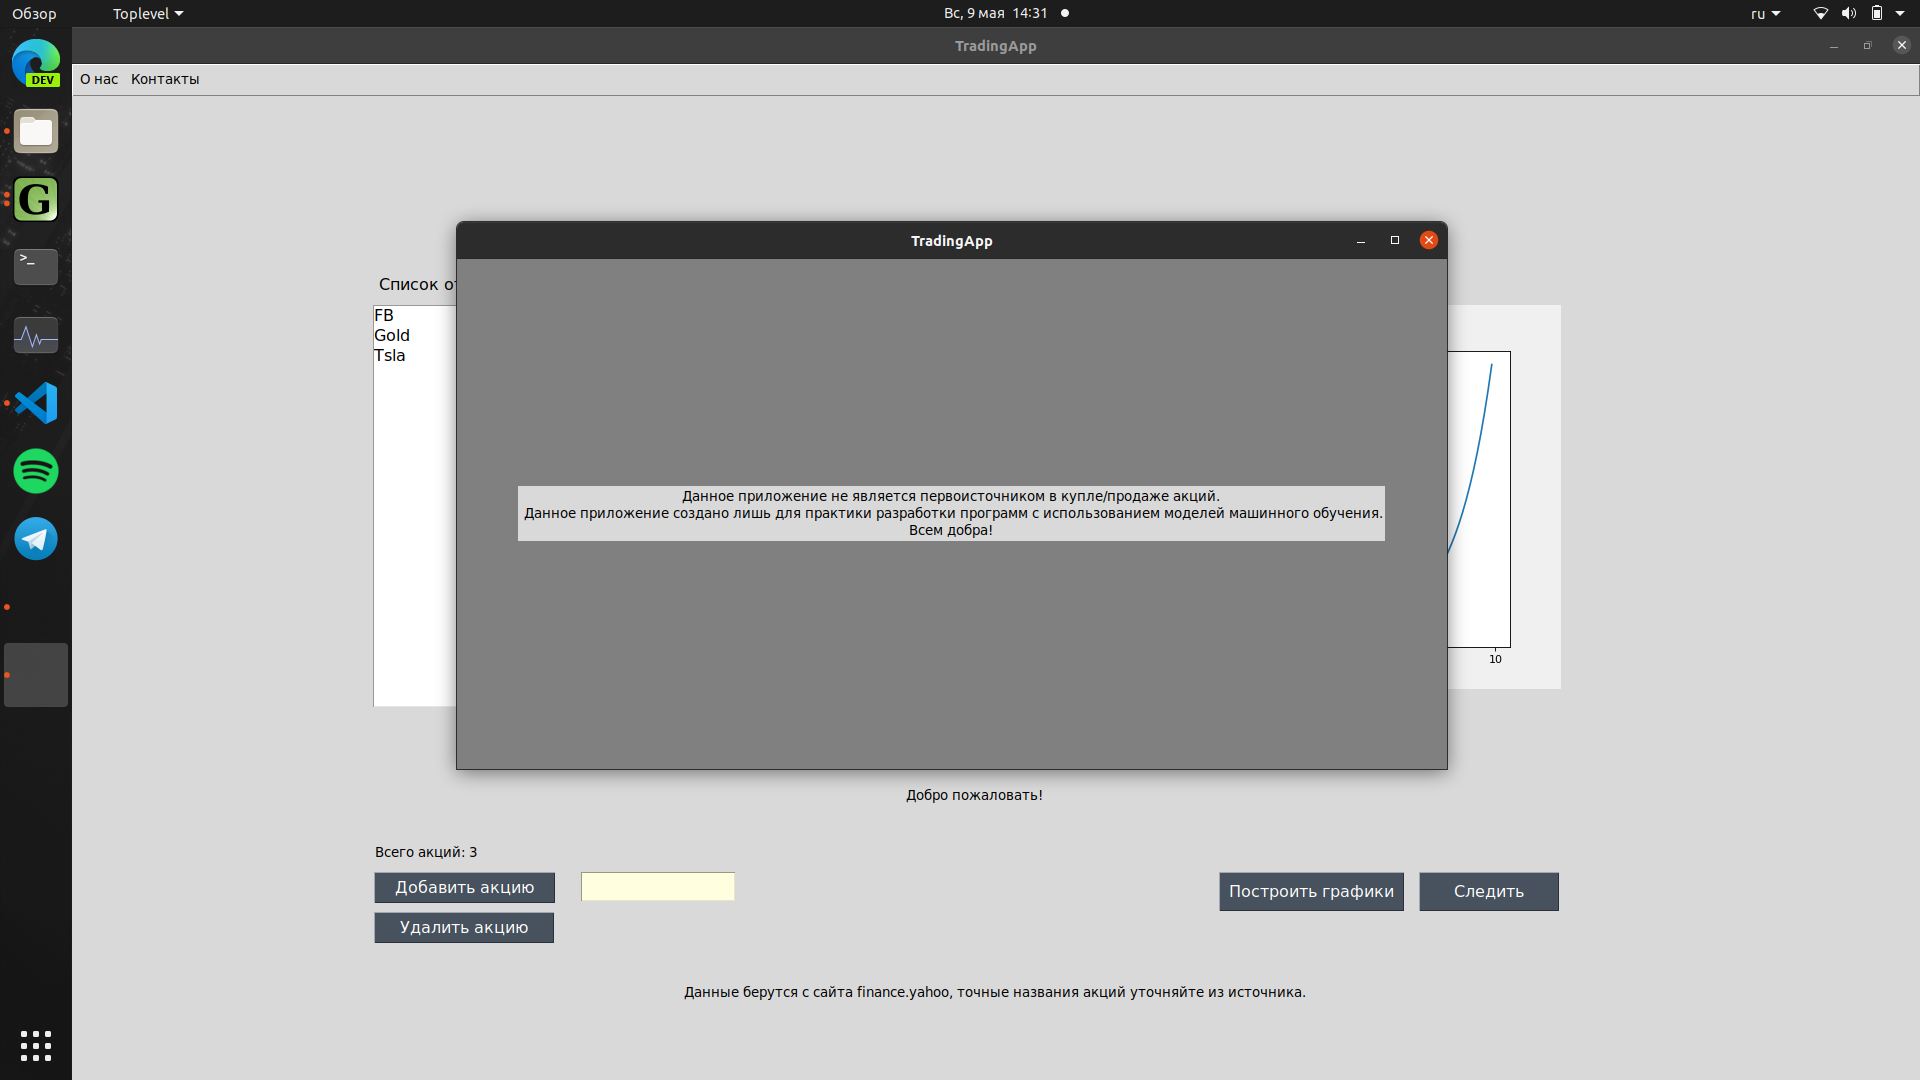
\includegraphics[scale=0.176]{About.png}
\end{frame}

\begin{frame}
 \frametitle{Интерфейс приложения:}
 Контакты:\\
 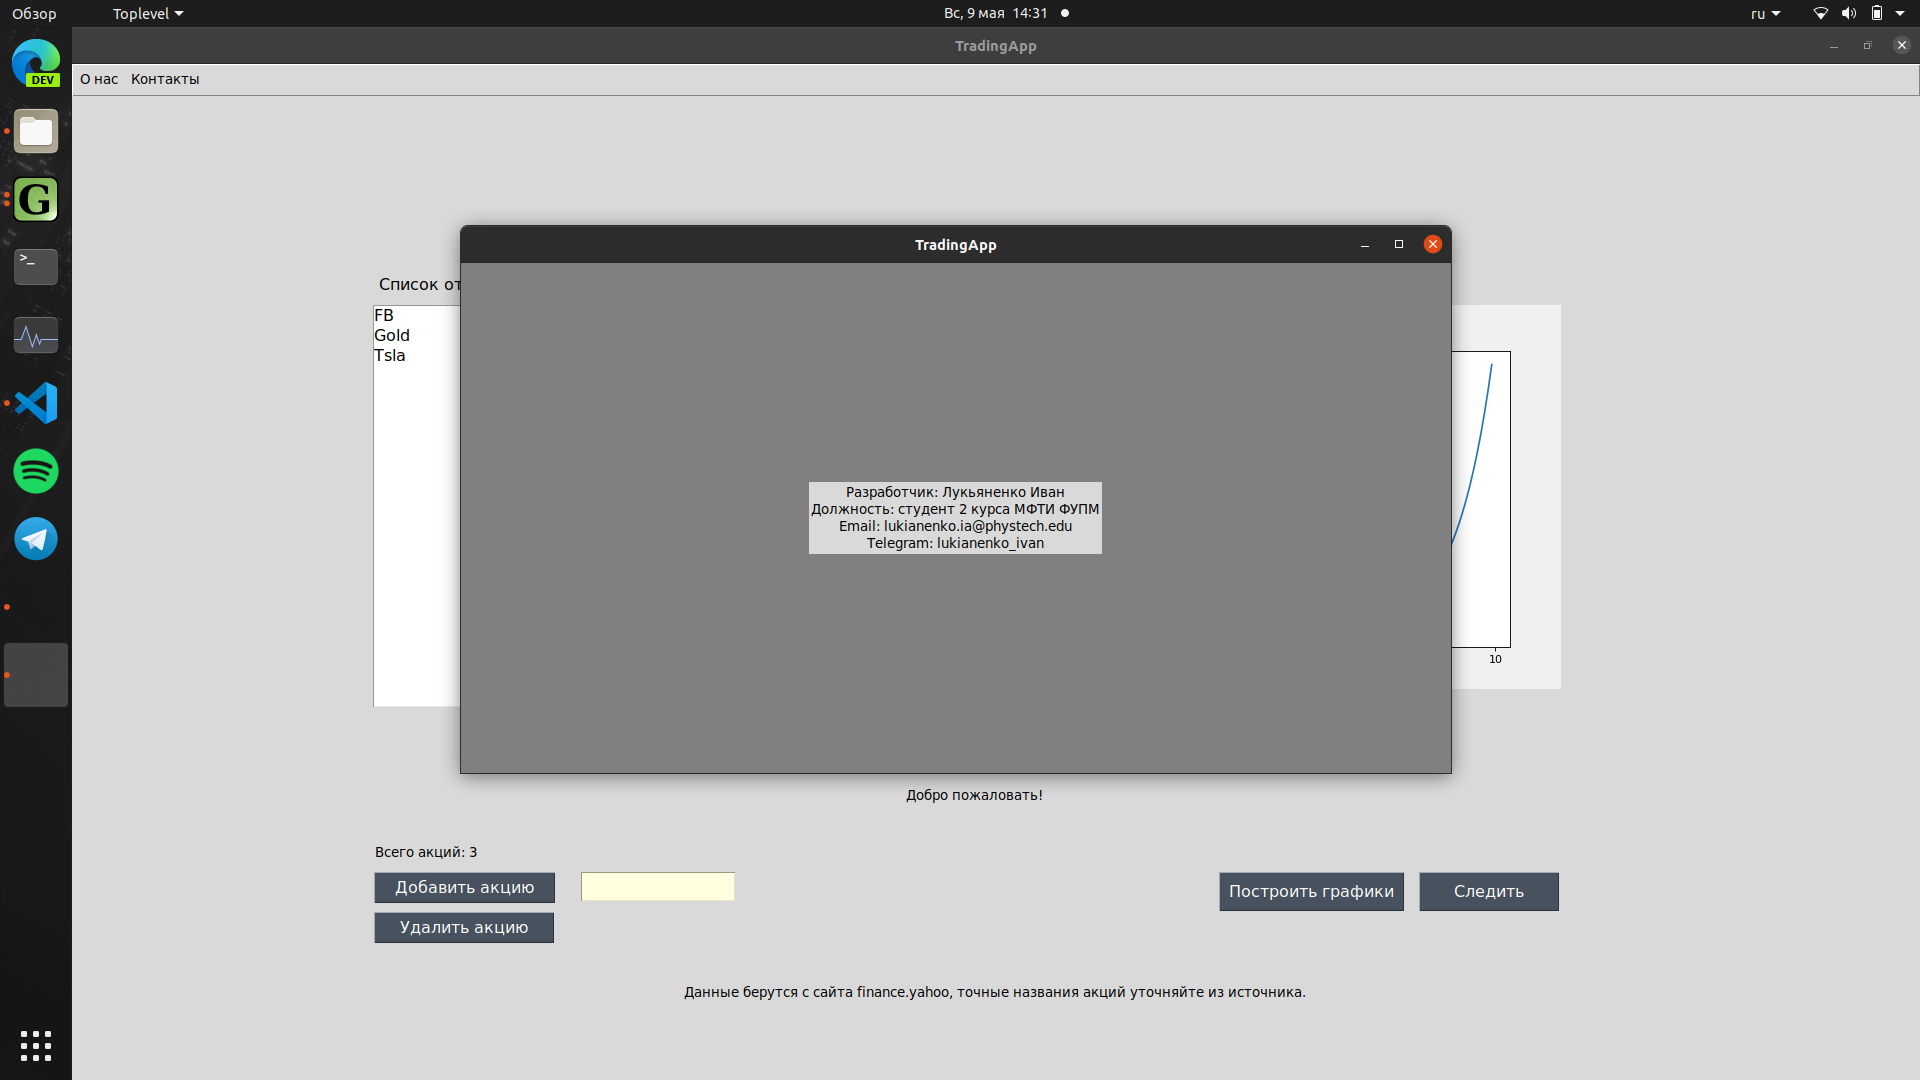
\includegraphics[scale=0.176]{Contacts.png}
\end{frame}

\begin{frame}
 \frametitle{Интерфейс приложения:}
 Окно ожидания\\
 \includegraphics[scale=0.176]{NNlearning.png}
\end{frame}

\begin{frame}
 \frametitle{Интерфейс приложения:}
 Рассмотрим основное окно:
 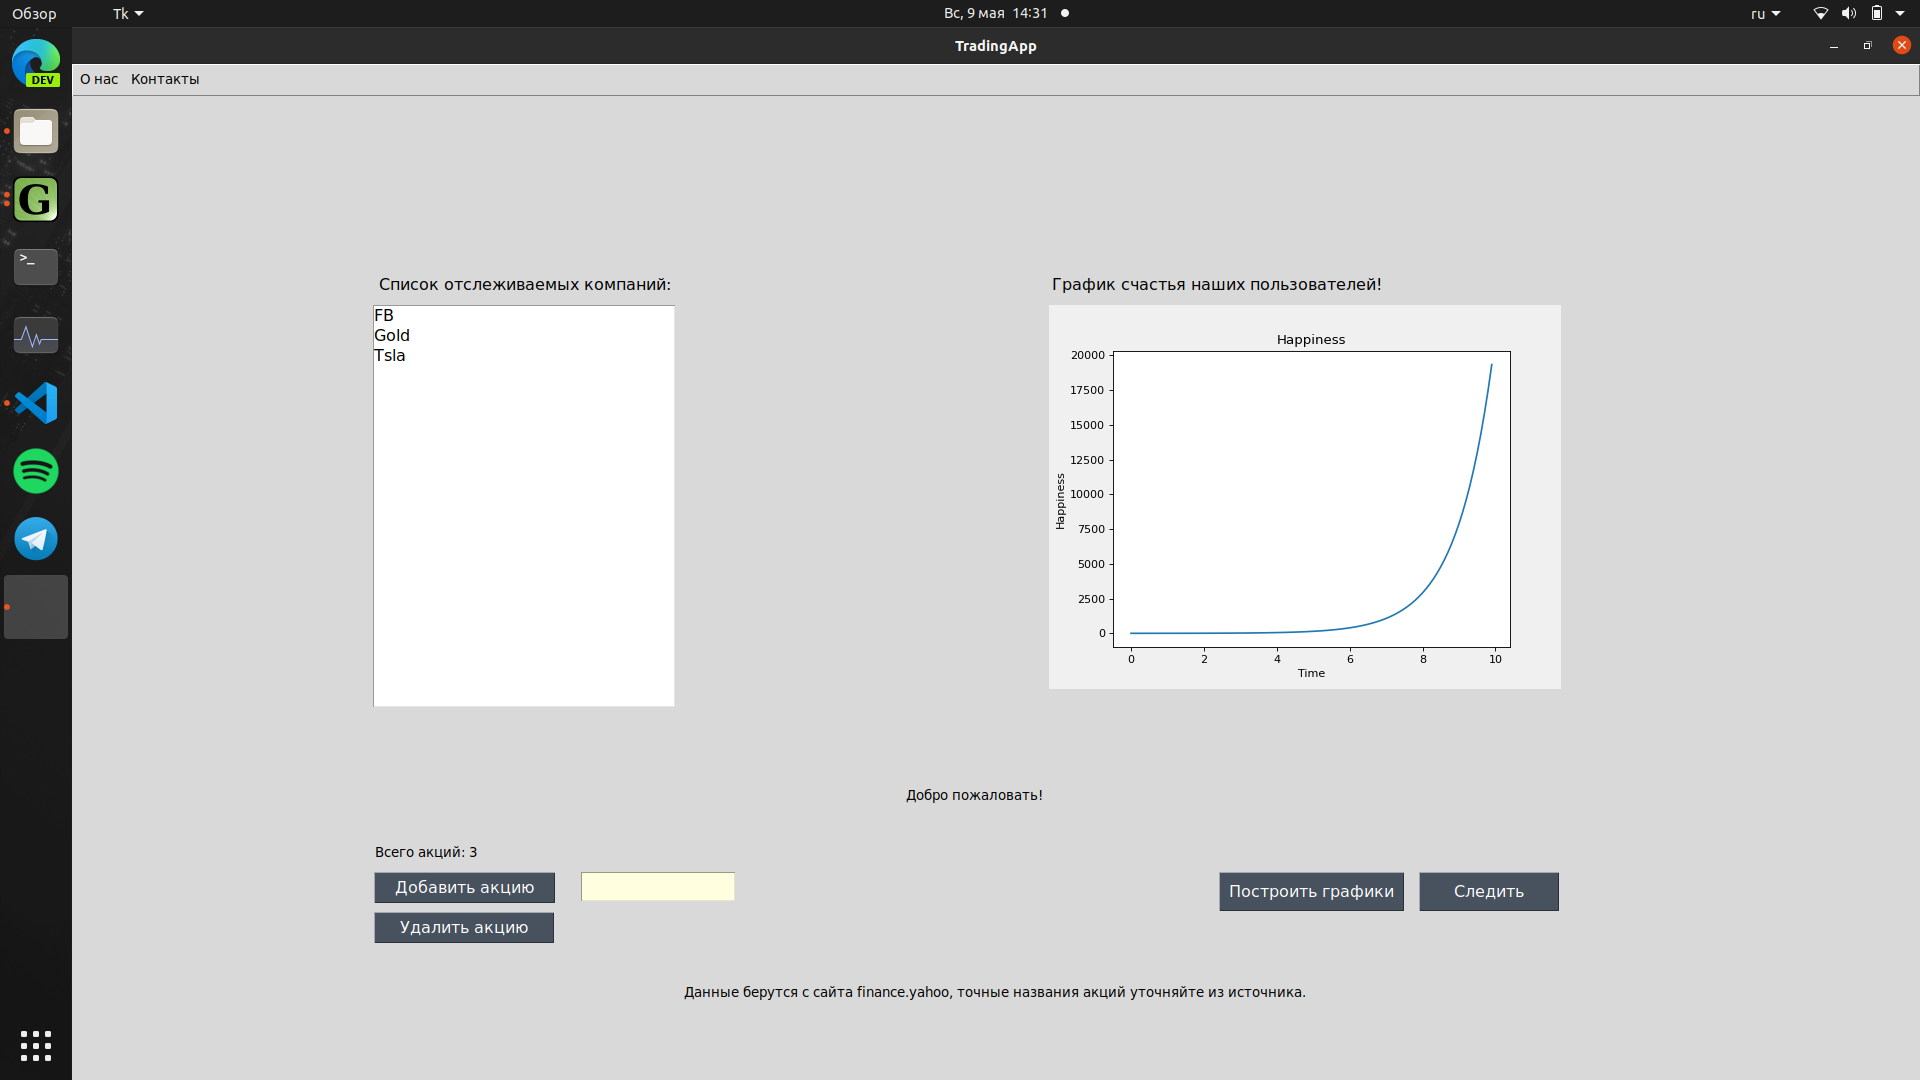
\includegraphics[scale=0.176]{mainWindow.png}
\end{frame}

\begin{frame}
 \frametitle{Интерфейс приложения:}
 В верхнем меню находятся две кнопки \textbf{О нас} и \textbf{Контакты}, которые cоздают соответсвующие окна.\\
 В левой части окна находится \textbf{Список отслеживаемых компаний:}\\
 Ниже находятся две кнопки \textbf{Добавить акцию} и \textbf{Удалить акцию}. 
 Рядом с первой кнопкой поле для ввода текста, чтобы пользователю добавить акцию нужно ввести название(уточнить в источнике название) и нажать кнопку \textbf{Добавить}.\\
 Чтобы удалить акцию, необходимо выделить акцию в списке и нажать на копку \textbf{Удалить акцию}\\
\end{frame}
\begin{frame} 
 \frametitle{Интерфейс приложения:}
 В правой части окна находится \textbf{График} отслеживаемой акции, по нажатии на акцию в списке, показывается ее график и прогноз.\\
 Кнопка \textbf{Следить} отвечает за создание и обучение нейросетей для акций из \textbf{Списка отслеживаемых акций} и запускается окно ожидания\\
 Кнопка \textbf{Построить графики} отвечает за построение актуальных графиков стоимости.\\
 В середине находится \textbf{NotificationBox}, в котором показывается готовность графиков или нейронных сетей.
\end{frame}

\begin{frame}
 \frametitle{Нейронная сеть:}
 В модуле NN.py вы можете подробней ознакомится с кодом для создания нейронной сети\\
 В проекте используется \textbf{7 слойная Рекурентная нейронная сеть} для анализа временных рядов.\\
 Почему используем именно \textbf{RNN}?\\
 Потому что временной ряд имеет свойство \textbf{памяти}, поэтому наша модель должна в некотором смысле обладать некоторым эффектом запоминания.\\
 Используемая здесь модель показывает достаточное качество, я мог подольше поработать над этим, чтобы улучшить качество, но я посчитал, что это проект по программированию, а не по машинному обучению.\\
\end{frame}
\end{document}
